\section{Νέος μικροελεγκτής}
\label{sec:example3}

Όπως και στο προηγούμενο παράδειγμα, έτσι και σε αυτό, σε περίπτωση που ο χρήστης θέλει να χρησιμοποιήσει κάποιον μικροελεγκτή για τον οποίο δεν υπάρχει υλοποίηση στην παρούσα εργασία, θα πρέπει να κάνει κάποια έξτρα βήματα.

Αυτή η περίπτωση επέκτασης, είναι λιγότερο χρονοβόρα από την προηγούμενη, καθώς το μόνο που χρειάζεται να γίνει από πλευράς του χρήστη, είναι να δημιουργήσει το αρχείο που γράφεται στην γλώσσα στην οποία αναπτύχθηκε στα πλαίσια της εργασίας, και περιγράφει την εκάστοτε συσκευή. Από κει και πέρα, εφόσον θέλει να χρησιμοποιήσει περιφερειακά που ήδη υποστηρίζονται, δε χρειάζεται τίποτα επιπλέον, καθώς ο κώδικας σε C που είναι απαραίτητος ώστε να λειτουργήσουν, είναι ήδη υλοποιημένος.

Έστω λοιπόν ότι ο χρήστης θέλει να χρησιμοποιήσει τον μικροελεγκτή WeMos D1 mini Pro ESP8266. Αν στο αρχείο (.con)\footnote{\url{https://github.com/robotics-4-all/2020_riot_mde_thanos_manolis/blob/master/test_connections/example3.con}} όπου δηλώνονται οι συνδέσεις του κάθε περιφερειακού με τον μικροελεγκτή, συμπεριλάβει τον ελεγκτή αυτόν, τότε η εντολή για την παραγωγή κώδικα θα επιστρέψει το μήνυμα που φαίνεται στο \autoref{fig:error_message3}, καθώς δεν υπάρχει έτοιμη υλοποίηση.

\begin{figure}[!ht]
	\centering
	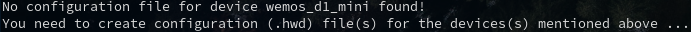
\includegraphics[width=0.8\textwidth]{./images/chapter6/error_message3.png}
	\caption{Μήνυμα για συσκευή που δεν υποστηρίζεται}
	\label{fig:error_message3}
\end{figure}

Άρα λοιπόν και πάλι ο χρήστης πρέπει να δημιουργήσει ένα .hwd αρχείο, όπου θα περιγράφει τα χαρακτηριστικά του μικροελεγκτή (σύμφωνα με τη γλώσσα που υλοποιήθηκε στην παρούσα εργασία). Αφού συμπληρωθεί αυτό το αρχείο\footnote{\url{https://github.com/robotics-4-all/2020_riot_mde_thanos_manolis/blob/master/riot_mde/supported_devices/boards/wemos_d1_mini.hwd}} με την κατάλληλη σύνταξη, τότε πλέον ο μικροελεγκτής αυτός υποστηρίζεται πλήρως, και άρα μπορεί να χρησιμοποιηθεί σαν όρισμα στη διαδικασία.